% Author: Victor Terron (c) 2013
% Email: `echo vt2rron1iaa32s | tr 132 @.e`
% License: CC BY-SA 4.0

\documentclass[14pt]{beamer}

\usepackage[utf8]{inputenc}
\usepackage{amsmath}
\usepackage{amsfonts}
\usepackage{amssymb}
\usepackage[spanish]{babel}
\usepackage{listings}
\usepackage{eurosans}
\usepackage{bold-extra}
\usepackage{caption}
\usepackage{eurosym}

\usetheme{Copenhagen}
\useoutertheme{infolines}
\setbeamercovered{dynamic}

% A Nice Title Page for Beamer Presentations
% http://github.com/dfalster/BeamerTitleSlide
\usepackage{tikz}
\usepackage[framemethod=tikz]{mdframed}

% Define a new mdframed environment
\newmdenv[tikzsetting={draw=black,fill=white,fill opacity=0.8},
  backgroundcolor=none,leftmargin=0,rightmargin=0, innertopmargin=4pt,
  skipbelow=\baselineskip, skipabove=\baselineskip]{TitleBox}

\lstset{basicstyle=\ttfamily,language=python}

\newcommand{\ShowCurrentSection}[0]{
  \AtBeginSection[]{
  \begin{frame}
      \frametitle{Índice}
      \begin{columns}
        \column{.4\textwidth}
          \begin{flushright}
            
\includegraphics[width=3cm]{pics/torvalds-to-nvidia.jpg}
          \end{flushright}
        \column{.5\textwidth}
          \tableofcontents[currentsection]
      \end{columns}
  \end{frame}}
}

\title{¡Sed Hackers!}
\author{Víctor Terrón}
\date{22 de mayo de 2013}
\institute{IAA-CSIC}

\begin{document}

{
\usebackgroundtemplate{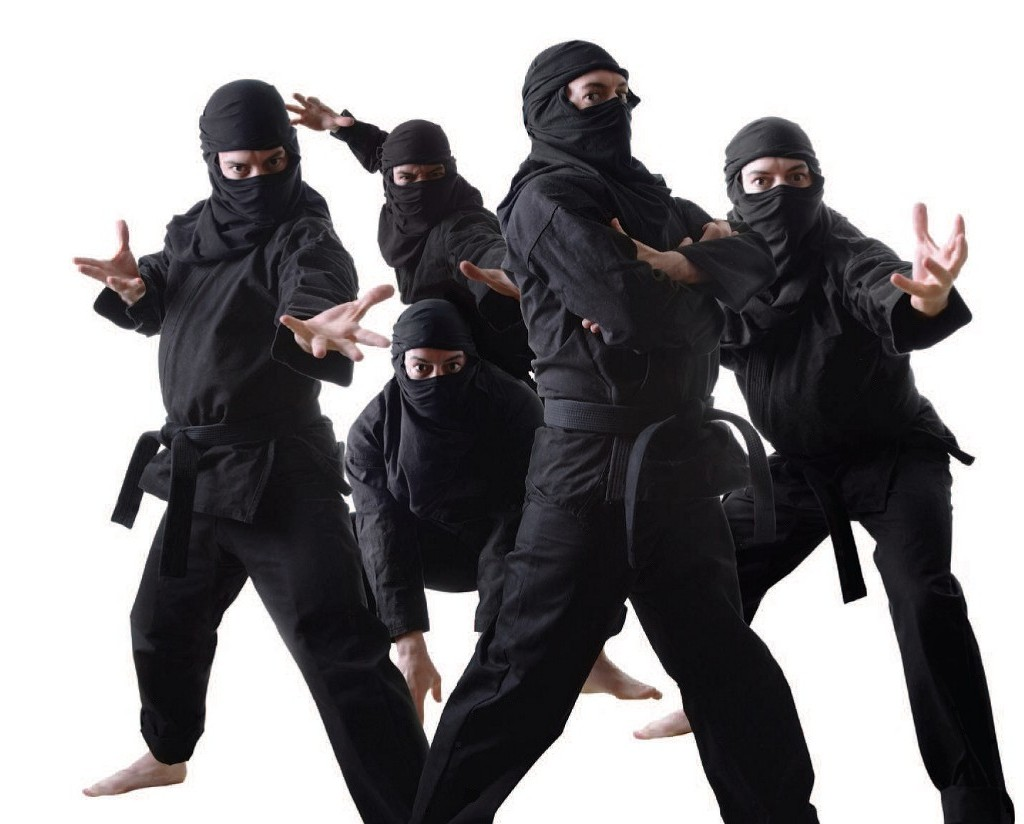
\includegraphics[height=1.0\paperheight]{pics/ninjas.jpg}}

\begin{frame}[plain]
  \vspace{6.25cm}
  \begin{TitleBox}
    {\LARGE \inserttitle} \\
    {\small \insertauthor \enspace --- \thinspace \url{http://github.com/vterron}}
  \end{TitleBox}
\end{frame}
}

\section{Introducción}
\begin{frame}{}
\begin{block}{}
    \centering \Large Las tres salidas después de la \structure{\tt ETSIIT}
\end{block}
\end{frame}

\begin{frame}{Tierra}
  \begin{center}
    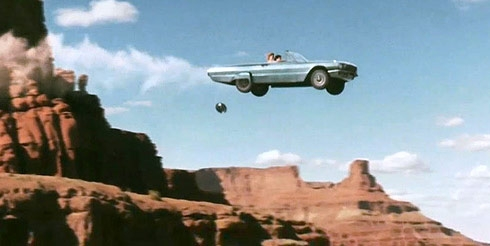
\includegraphics[width=0.6\textwidth]{pics/thelma-louise-cliff.jpg}
  \end{center}
\end{frame}

\begin{frame}{Mar}
  \begin{center}
    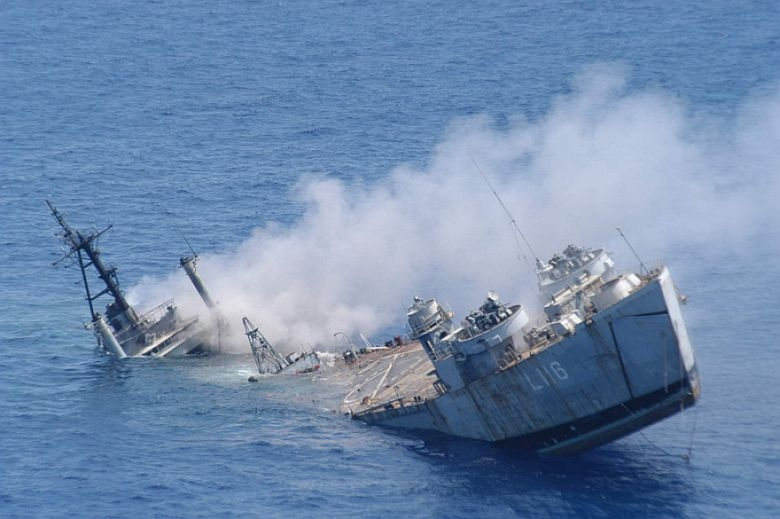
\includegraphics[width=0.6\textwidth]{pics/ship-sinking.jpg}
  \end{center}
\end{frame}

\begin{frame}{Aire}
  \begin{center}
    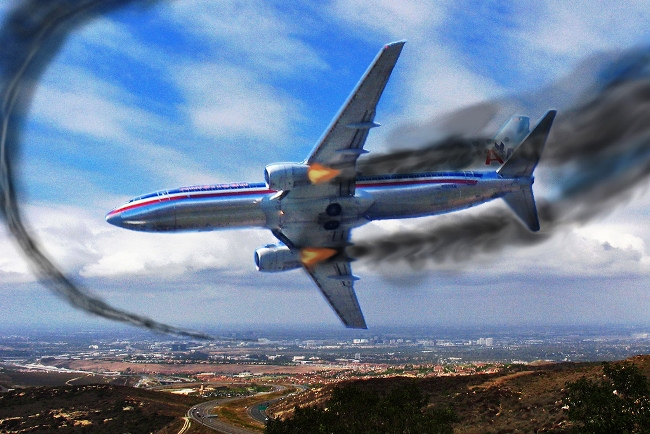
\includegraphics[width=0.6\textwidth]{pics/plane-crashing.jpg}
  \end{center}
\end{frame}

\begin{frame}{}
\begin{block}{}
    \centering \Large El destino de muchos: \structure{\tt consultoría}
\end{block}
\begin{figure}
  \centering
  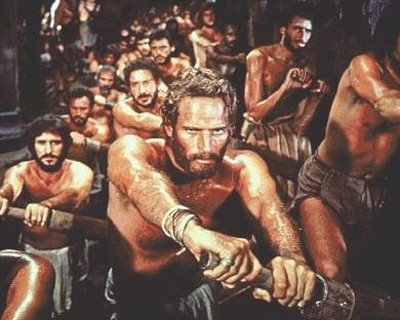
\includegraphics[width=0.4\textwidth]{pics/ben-hur-rowing.jpg}
  \caption*{Accenture, Northgate Arinso y demás cárnicas}
\end{figure}
\end{frame}

\begin{frame}{ETSIIT: A New Hope}
  \begin{itemize}
    \item Hay vida más allá de \structure{Arinso}
    \item Hay países donde la gente joven encuentra trabajo
    \item El ejemplo más evidente es \structure{Silicon Valley} \\
      {\small Empresas líder en el sector, proyectos muy interesantes
        y unas condiciones laborales impensables aquí en España}
    \item Todos querríamos \structure{trabajar} en una empresa así
    \item ¿Cuál es el \structure{perfil} de aquellos que lo consiguen?
  \end{itemize}
  \begin{center} \Large \bf ¡Todos son hackers!\end{center}
\end{frame}


\begin{frame}{Hackers}
    \begin{center}
      Hackers, por supuesto, en su \structure{verdadero significado}
    \end{center}

    \begin{block}{\footnotesize Definición según Wikipedia}
      \centering \footnotesize A person who enjoys \structure{exploring the
        limits of what is possible}, in a spirit of playful
      cleverness. They may also heavily modify software or hardware of
      their own computer system. It includes building, rebuilding,
      modifying, and creating software, or anything else, either to
      \structure{make it better} or faster or to give it added
      features or to \structure{make it do something it was never
        intended to do}.
    \end{block}

  \begin{itemize}
    \item \href{http://www.catb.org/esr/faqs/hacker-howto.html}
      {\structure{How To Become A Hacker}}, de Eric Raymond
    \item A todos los hackers les \structure{apasiona} la programación
  \end{itemize}
\end{frame}


\begin{frame}{}
  \vspace{2cm}
  \begin{alertblock}{}
    \centering Porque a todos nos apasiona programar... \textbf{¿verdad?}
  \end{alertblock}
  \begin{center}
    
\includegraphics[width=5cm]{pics/you_dont_say.png}
  \end{center}
\end{frame}

\begin{frame}{}
  \begin{center}
    
\includegraphics[width=0.8\textwidth]{pics/nothing-to-do-here.jpg}
  \end{center}
\end{frame}

\begin{frame}{Hacker = programador}
\begin{itemize}
\item La programación es \structure{fundamental} en este gremio
\item Idea \structure{absurda}: \emph{``Los ingenieros no programan''}
\item No sólo lo hacen, sino que son \structure{mejores} que nadie
\item La alternativa es ser... un \structure{powerpoinista}.
\item \href{http://www.alfredodehoces.com/fuckowski-on-line}
      {\structure{Fuckowski}, memorias de un ingeniero}
\end{itemize}
\end{frame}

\begin{frame}{}
  \begin{center}
    
\includegraphics[width=0.6\textwidth]{pics/the-oatmeal-real-geeks.jpg}
  \end{center}
\end{frame}

\begin{frame}{}
\begin{itemize}
  \item Existen empresas como Valve, Twitter o GitHub
  \item Sin \structure{horarios} ni código de \structure{vestimenta}
  \item El salario medio en Twitter es de \structure{\$115,809} (¡!)
  \item Valve es un paradigma de \structure{organización horizontal}
  \item \href{http://www.valvesoftware.com/company/Valve_Handbook_LowRes.pdf}
        {\structure{Manual del nuevo empleado de Valve}}
  \item Aspirad a trabajar en un sitio así
  \item Aspirad a ser \structure{hackers}
\end{itemize}
\end{frame}

\ShowCurrentSection

\setbeamerfont{itemize/enumerate body}{size=\footnotesize}

\section{Y éste quién es}
\begin{frame}{Quién soy}
\begin{itemize}
  \item Víctor Terrón
  \item \url{http://www.github.com/vterron}
  \item Ingeniería Informática (2003-2009)
  \item \structure{Hijos de Eva} — Apuntes de Fundamentos Físicos
  \item Intercambio en Irlanda (\structure{Erasmus}) y EE.UU. (\structure{programa propio})
  \item Instituto de Astrofísica de Andalucía (CSIC)
  \item Desarrollo software para \structure{instrumentos astronómicos}
  \item En ocasiones soy \structure{operador de telescopio} en Calar Alto
  \item Desde 2009, \structure{semanas después} de terminar la carrera
\end{itemize}
\end{frame}

\begin{frame}{1.23m CAHA}
  \begin{center}
    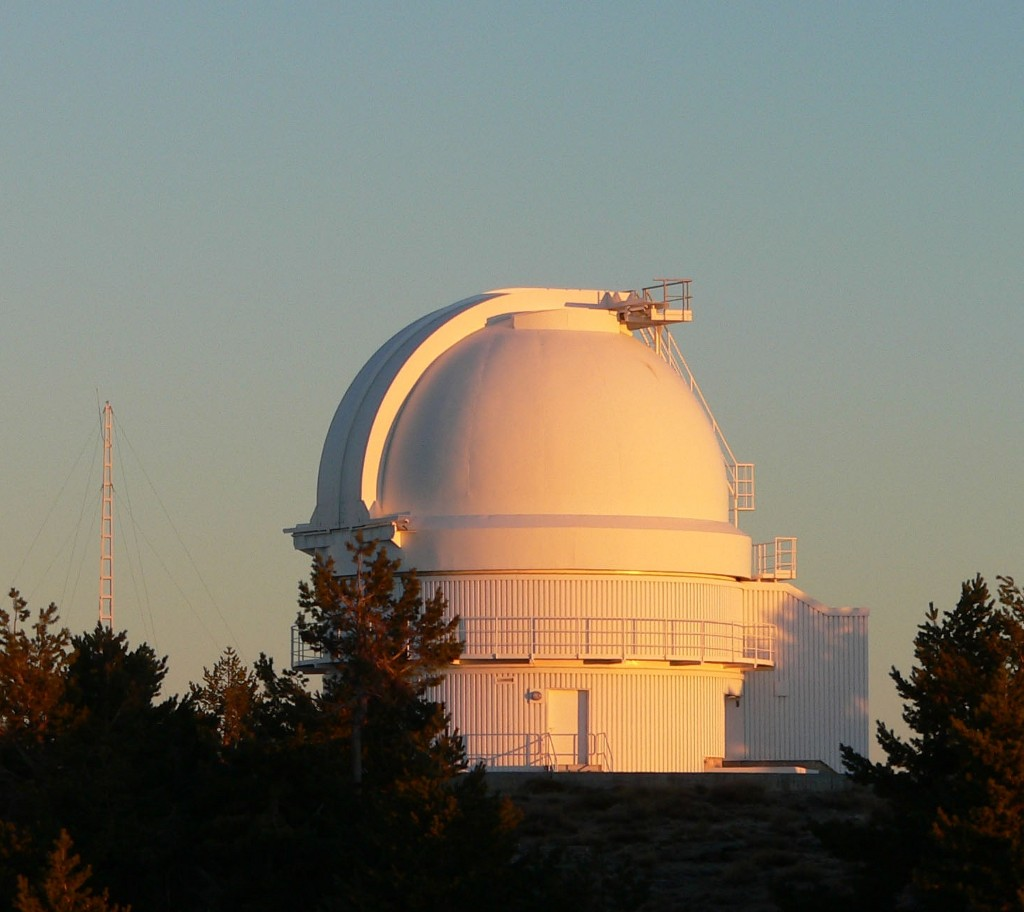
\includegraphics[height=0.8\textheight]{pics/123m_CAHA_1.jpg}
  \end{center}
\end{frame}

\begin{frame}{1.23m CAHA}
  \begin{center}
    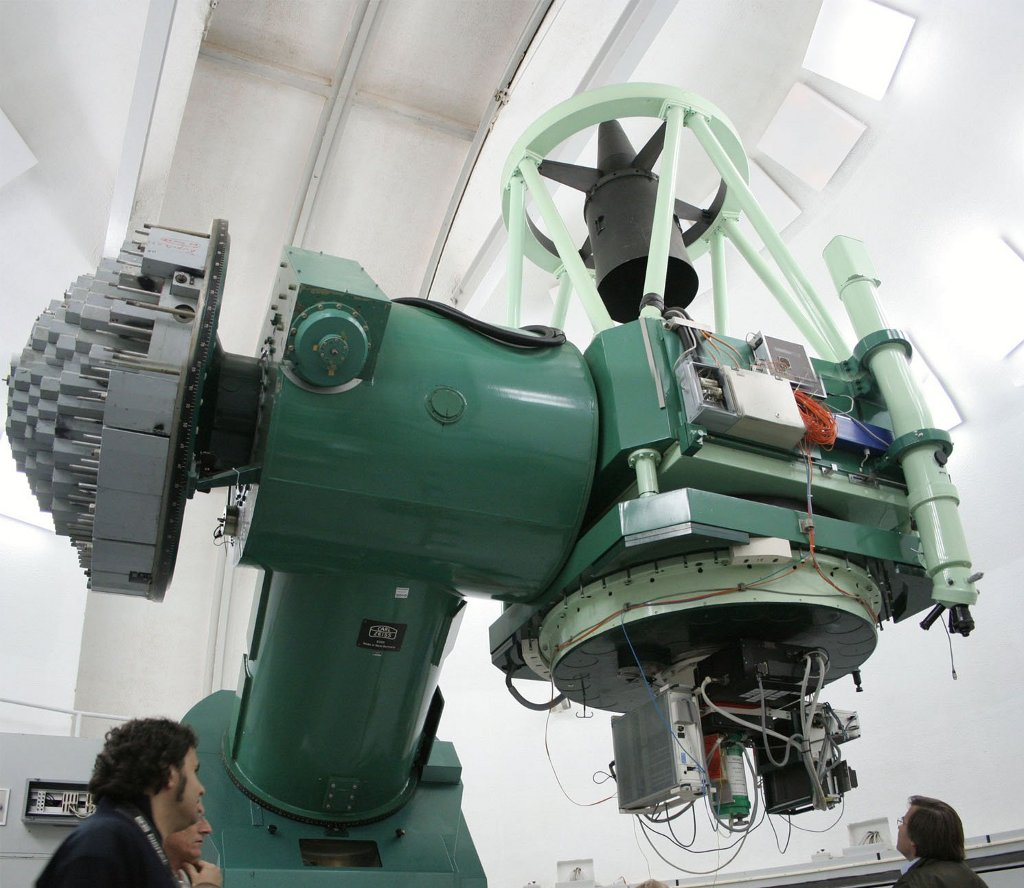
\includegraphics[height=0.8\textheight]{pics/123m_CAHA_2.jpg}
  \end{center}
\end{frame}

\setbeamerfont{itemize/enumerate body}{size=\small}

\begin{frame}{¿Y eso?}
\begin{itemize}
  \item La pregunta es \structure{por qué me cogieron a mí}, y no a otro
  \item En última instancia, buscaban dos cosas en un candidato:
     \begin{itemize}
       \item Que supiera de \structure{GNU/Linux}
       \item Y hablara \structure{inglés}
     \end{itemize}
  \item Y ésas eran básicamente las únicas dos cosas que yo sabía
  \item \structure{Smart and Gets Things Done}, de Joel Spolsky
\end{itemize}
  \begin{alertblock}{\centering Primer Axioma}
    \centering El expediente sólo sirve para que te den becas
  \end{alertblock}
\end{frame}

\setbeamerfont{itemize/enumerate body}{size=\footnotesize}

\begin{frame}{}
  \begin{block}{}\centering
    \Large \structure{GNU/Linux}
  \end{block}
  \begin{itemize}
    \item El manejo de la línea de comandos es \structure{esencial}
    \item La curva de aprendizaje es suave (es decir, muy difícil)
    \item No será \structure{cómodo} al principio, ni agradable
    \item \emph{¿No acabaría antes....?} Respuesta: \structure{sí}
    \item Pero aprenderéis muchísimo — incontables conceptos
    \item La abstracción de las GUI nos \structure{limitan intelectualmente}
    \item No seáis otra \structure{Generación XP}
    \item \structure{In the Beginning... Was the Command Line}, de  Neal Stephenson
  \end{itemize}
\end{frame}

\begin{frame}{}
  \begin{block}{}\centering
    \Large \structure{Inglés}
  \end{block}
  \begin{itemize}
    \item El 99\% del material existente \structure{está en la lingua franca}
    \item El 1\% restante son traducciones del inglés (por ejemplo, Wikipeadia)
    \item Las de arriba son cifras inventadas, pero captáis el mensaje
    \item Estudiad como sea al menos un año en \structure{un país de habla inglesa}
    \item A ser posible \structure{el último curso} (para no volver después)
    \item Empezad a ahorrar ya si hace falta, aunque \structure{tampoco necesitáis tanto}
    \item Yo gasté \EUR{8,500} en \structure{un curso entero} en California
    \item Necesitáis un título: \structure{Certificate of Advanced English}
    \item El \structure{First} está bien cuando tienes quince años
  \end{itemize}
\end{frame}

\section{¿Y vosotros?}
\begin{frame}{Los años que os quedan}
  \begin{itemize}
    \item Tenéis por delante unos años \structure{bastante feos} en la ETSIIT
    \item Los profesores buenos con \structure{escasísimos}, y muy valiosos.
    \item Los mediocres o directamente \structure{inútiles abundan}, y
      se reproducen a una velocidad asombrosa. Parecen destinados a
      dominar el mundo.
    \item Consejo: centrad vuestros esfuerzos en los pocos docentes e
      investigadores que \structure{merecen la pena}.
    \item El mundo ya está lleno de gente que \structure{se limitó a
      aprobar asignaturas}, incluso con buena nota.
  \end{itemize}

  \begin{alertblock}{\centering Segundo Axioma}
    \centering No hay asignaturas difíciles, sólo malos profesores
  \end{alertblock}
\end{frame}

\begin{frame}{Carpe Diem}
  \begin{itemize}
    \item No quiero sonar como un viejo, ¡pero \structure{aprovechad
      el tiempo}!
    \item WoW, LoL, Facebook, Tuenti, Cuánto Cabrón o Series Yonkis
    \item Los que dediquéis todo ese tiempo a esfuerzos creativos
      seréis \structure{expertos con varios años de experiencia} para
      cuando obtengáis el título.
    \item El resto empezaréis a aprender en serio \structure{sólo
      entonces}, y estaréis como mínimo varios años por detrás de los
      que hiceron algo más que ir a clase, prácticas y exámenes.
    \item Todos los hackers se caracterizan por \structure{aprovechar
      muy bien el tiempo}. Hay tiempo para todos los proyectos que os
      propongáis.
    \item No gastéis esfuerzos en \structure{conocimientos inútiles}
      como saberos al dedillo cuáles son los últimos modelos en
      tarjetas gráficas. Dentro de 50 años se \structure{seguirá
        programando en Fortran y C}, pero no habrá APIs para Facebook.
    \item ¡Vamos a hacer cosas!
  \end{itemize}
\end{frame}

\setbeamerfont{itemize/enumerate body}{size=\normalsize}

\section{How to Become a Ninja}

\ShowCurrentSection

\begin{frame}{Vale... ¿pero cómo?}
  \begin{itemize}
    \item Empezad usando GNU/Linux como \structure{único sistema
      operativo}, para todo
    \item Aprended sólidamente los fundamentos de la programación, y
      de aquí a cinco años proponéos dominar {\bf al menos} tres
      lenguajes:
         \begin{itemize}
           \item Uno de \structure{bajo} nivel (C o C++)
           \item Uno de \structure{alto} (Python o Perl)
           \item Y uno \structure{\emph{raro}} (Lisp o Erlang)
         \end{itemize}
    \item Expresarse \structure{con fluidez} en inglés es esencial.
    \item No olvidéis el \structure{perfil blando}: música, artes
      marciales.
    \item Nunca preguntéis \emph{``¿Y esto para qué sirve?''}
   \end{itemize}
\end{frame}

\setbeamerfont{itemize/enumerate body}{size=\small}

\begin{frame}{Software Libre}

   \begin{block}{}\centering
    \normalsize Involucraos en un proyecto de software libre.
   \end{block}

   \begin{itemize}
     \item Por más que algunos profesores que tendréis discrepen
     \item No hay nada que \structure{impresione} más en un currículum
     \item Encontrad \structure{un proyecto que os guste}, y empezad poco a poco
     \item Parches muy pequeños al principio
     \item Podéis empezar con \structure{traducciones}, si lo preferís
     \item Launchpad (Ubuntu) o GitHub
   \end{itemize}
\end{frame}

\begin{frame}{Titulitis}
  \begin{itemize}
    \item No sois \emph{``Ingenieros superiores''}
    \item Incluso \emph{``Ingeniero''} a secas son palabras mayores
    \item No lo planteéis jamás como un \structure{Ingenieros} vs
      \structure{FPs}
    \item Telecomunicaciones mola porque aprenden más \structure{Física}
    \item El título es sólo \structure{un trozo de papel}
    \item Tenéis la obligación moral de ser \structure{humildes}
  \end{itemize}

  \begin{alertblock}{\centering Tercer Axioma}
    \centering Los de FP probablemente os dan mil vueltas
  \end{alertblock}
\end{frame}



\begin{frame}{git \textgreater svn}

  \begin{alertblock}{\centering Primer Mandamiento}
    \centering ¡No uséis Subversion!
  \end{alertblock}

  \begin{itemize} \itemsep0em
    \item Usad sistemas de control de versiones \structure{distribuidos}
    \item Mercurial o Git, ya es una cuestión de gustos
  \end{itemize}

  \begin{block}{}\centering
    \scriptsize For the first 10 years of kernel maintenance, we
    literally used tarballs and patches, \structure{which is a much
      superior source control management system than CVS is}, but I
    did end up using CVS for 7 years at a commercial company and I
    hate it with a passion. When I say I hate CVS with a passion, I
    have to also say that if there are any SVN (Subversion) users in
    the audience, you might want to leave. Because my hatred of CVS
    has meant that \structure{I see Subversion as being the most
      pointless project ever started}. The slogan of Subversion for a
    while was \emph{CVS done right}, or something like that, and if
    you start with that kind of slogan, there's nowhere you can
    go. There is no way to do CVS right.
  \end{block}
  \vspace{-0.5cm}
  \begin{center} \scriptsize Linus Torvalds (2007) \end{center}
\end{frame}

\begin{frame}{Dijkstra}
   \begin{block}{}\centering
   \normalsize The teaching of BASIC should be rated as
   a criminal offence: it mutilates the mind beyond recovery.
   \end{block}
  \vspace{-0.5cm}
  \begin{center} \scriptsize Edsger W. Dijkstra (1984) \end{center}

  \begin{figure}
    \centering
    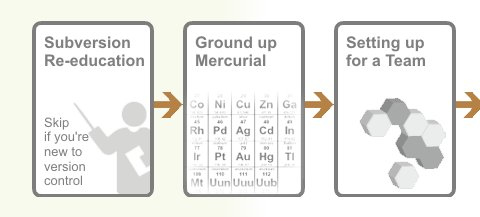
\includegraphics[width=0.45\textwidth]{pics/svn-reeducation.jpg}
    \caption*{\url{http://hginit.com/}}
  \end{figure}
\end{frame}

\begin{frame}{Emacs}

  \begin{block}{\scriptsize Neal Stephenson} \centering
    \scriptsize I use Emacs, which might be thought of as a thermonuclear word processor.
  \end{block}

  \begin{block}{\scriptsize Eric S. Raymond} \centering
    \scriptsize Emacs is undoubtedly the most powerful programmer's editor in
    existence. It's a big, feature-laden program with a great deal of
    flexibility and customizability. [...] Emacs has an entire
    programming language inside it that can be used to write
    arbitrarily powerful editor functions.
  \end{block}

  \begin{itemize} \itemsep0em
    \item IDEs como \structure{Eclipse} son cómodas pero simplifican demasiado
    \item Aprended a operar a mano \structure{antes de usar una calculadora}
    \item \structure{Real Programmers} use Emacs! — \url{https://xkcd.com/378/}
  \end{itemize}

\end{frame}

\begin{frame}{Dos casos}

  \begin{exampleblock}{Escenario A}\centering
   \small Usar GMail a traver de su interfaz web
   \end{exampleblock}

  \begin{block}{Escenario B} \centering
    \small Descargar los correos electrónicos del servidor vía POP
    usando \structure{fetchmail}, procesarlos y almacenarlos en el
    directorio que corresponda con \structure{procmail}. Incorporar un
    script programado en \structure{Python} para que nos envíe un SMS
    si recibimos un e-mail importante o uno de nuestros discos duros
    empieza a dar síntomas de error y lo detectamos con
    \structure{smartctl}.
   \end{block}

  \begin{alertblock}{\centering Cuarto Axioma}
    \centering Difícil es más divertido
  \end{alertblock}

\end{frame}

\begin{frame}{GitHub}
  \begin{itemize}
    \item GitHub (o equivalente) es tu nuevo currículum
    \item Muestra de forma transparente \structure{qué has hecho, cómo y cuándo}
    \item Permite evaluar la \structure{calidad de tu código y contribuciones}
    \item Para las empresas buenas, esto es lo \structure{único que importa}
  \end{itemize}

  \begin{center}
    
\includegraphics[width=6cm]{pics/github-logo.png}
  \end{center}
\end{frame}

\begin{frame}{GitHub}

  \begin{block}{\scriptsize} \centering
    \Large Colgad en GitHub {\bf todo} lo que hagáis
  \end{block}

  \begin{itemize}
    \item Desde \structure{prácticas} a ficheros de configuración rc
    \item Siempre hay alguien a quien le serán útiles
    \item Devolved a la comunidad parte del esfuerzo
    \item Sed \structure{creadores} de contenidos, no sólo consumidores
  \end{itemize}

\end{frame}

\begin{frame}{}
  \begin{columns}
    \column{.6\textwidth}
    \begin{block}{}\centering\Large\bf
      ¿La mejor forma de \structure{aprender}?
    \end{block}
    \begin{center}
      \structure{\huge Hacer cosas \emph{guays} \textbf{sin pensar}}
    \end{center}
    \column{.4\textwidth}
    
\includegraphics[width=.9\textwidth]{pics/be-cool.jpg}
  \end{columns}
\end{frame}

\begin{frame}{Arduino}
  \begin{center}
  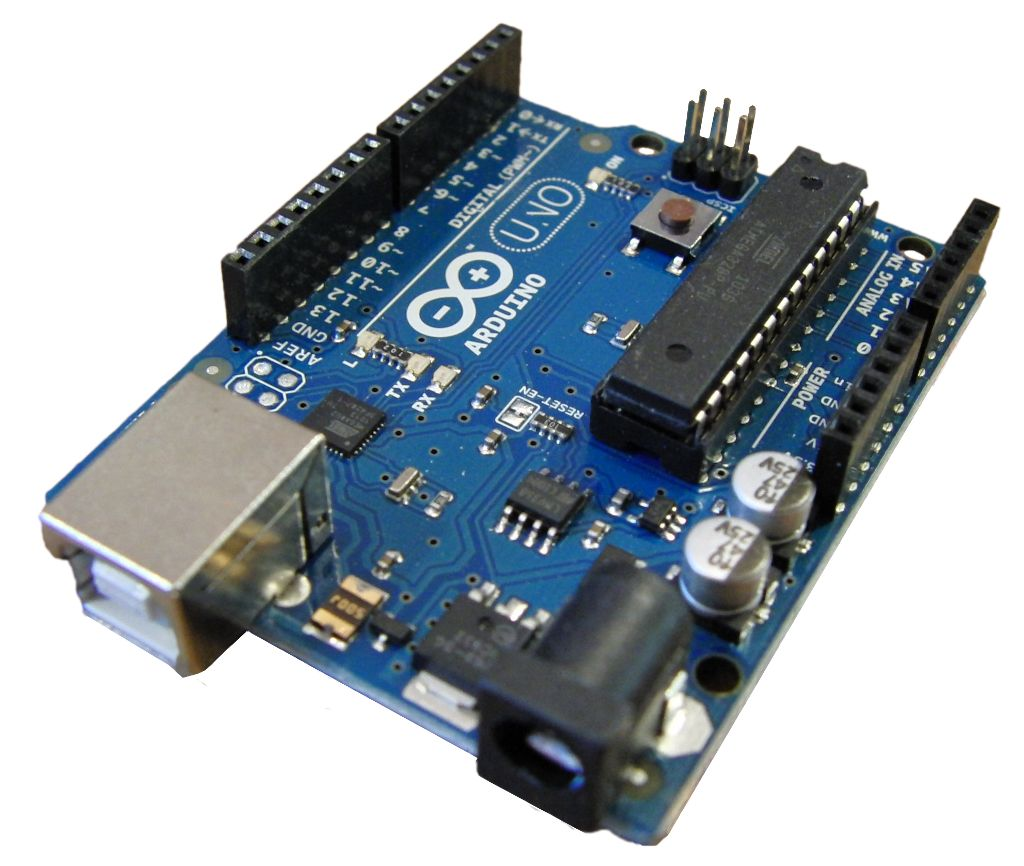
\includegraphics[width=.45\textwidth]{pics/arduino.jpg}
  \end{center}
  \vspace{-0.5cm}
  \begin{block}{}\centering
    Plataforma de hardware libre, basada en una placa con un
    microcontrolador y un entorno de desarrollo
  \end{block}
\end{frame}

\begin{frame}{Arduino: Tanque}
  \begin{figure}
    \centering
    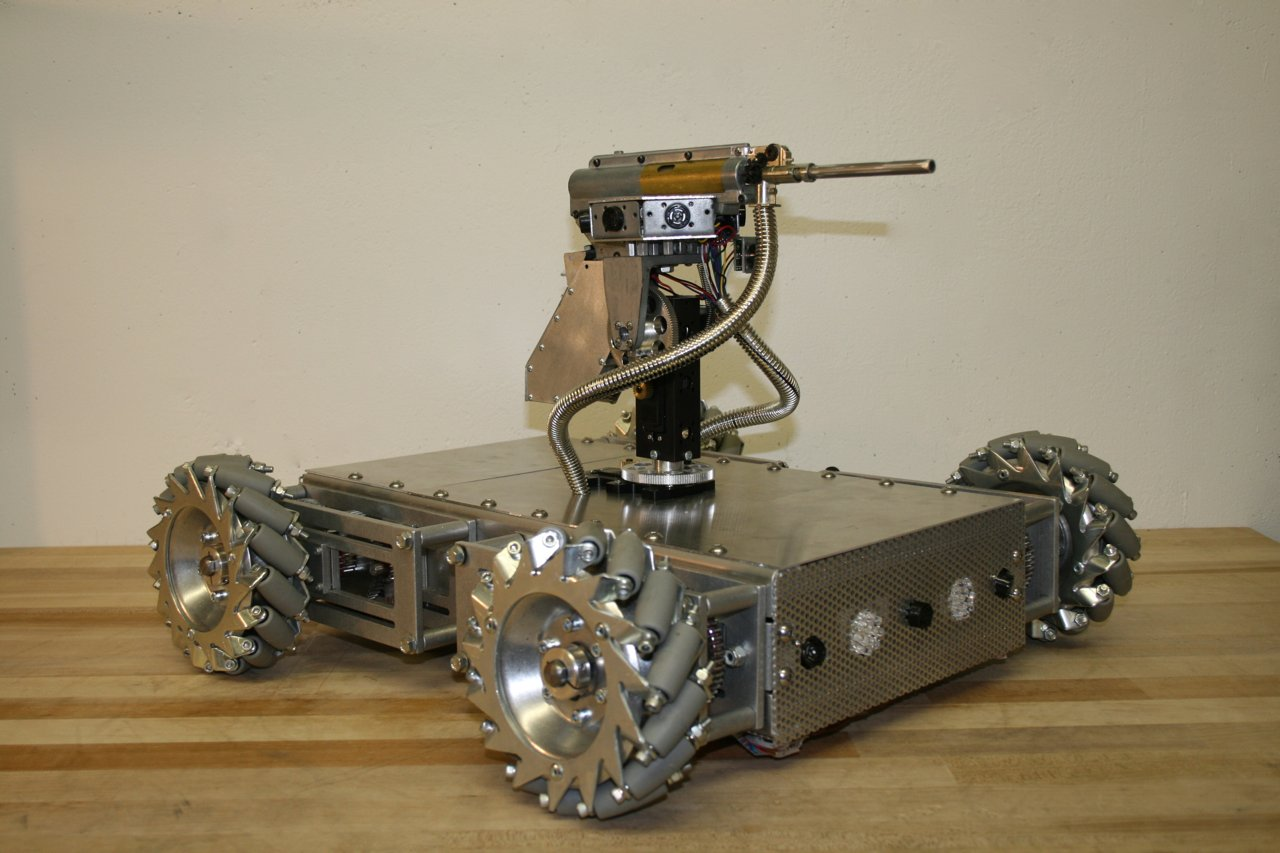
\includegraphics[width=0.8\textwidth]{pics/arduino-tank.jpg}
    \caption*{\small \url{http://beatty-robotics.com/mechatronic-tank/}}
  \end{figure}
\end{frame}

\begin{frame}{Arduino: Araña}
  \begin{figure}
    \centering
    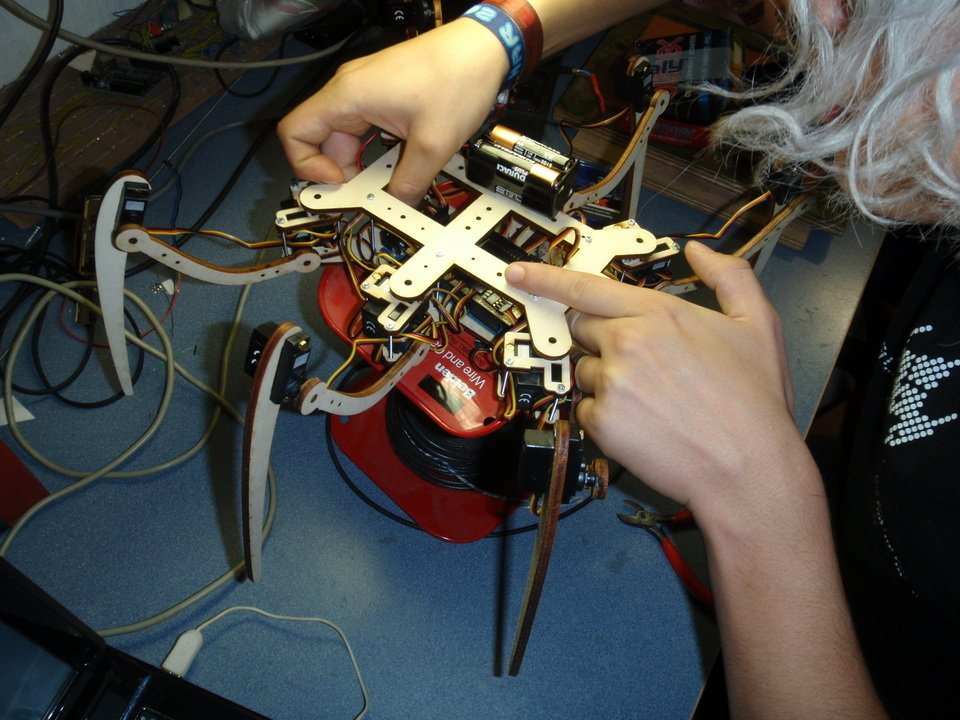
\includegraphics[width=0.7\textwidth]{pics/arduino-spider.jpg}
    \caption*{\small \url{http://www.flickr.com/photos/wizard23/3911240094/}}
  \end{figure}
\end{frame}

\begin{frame}{Arduino: Cuadricóptero}
  \begin{figure}
    \centering
    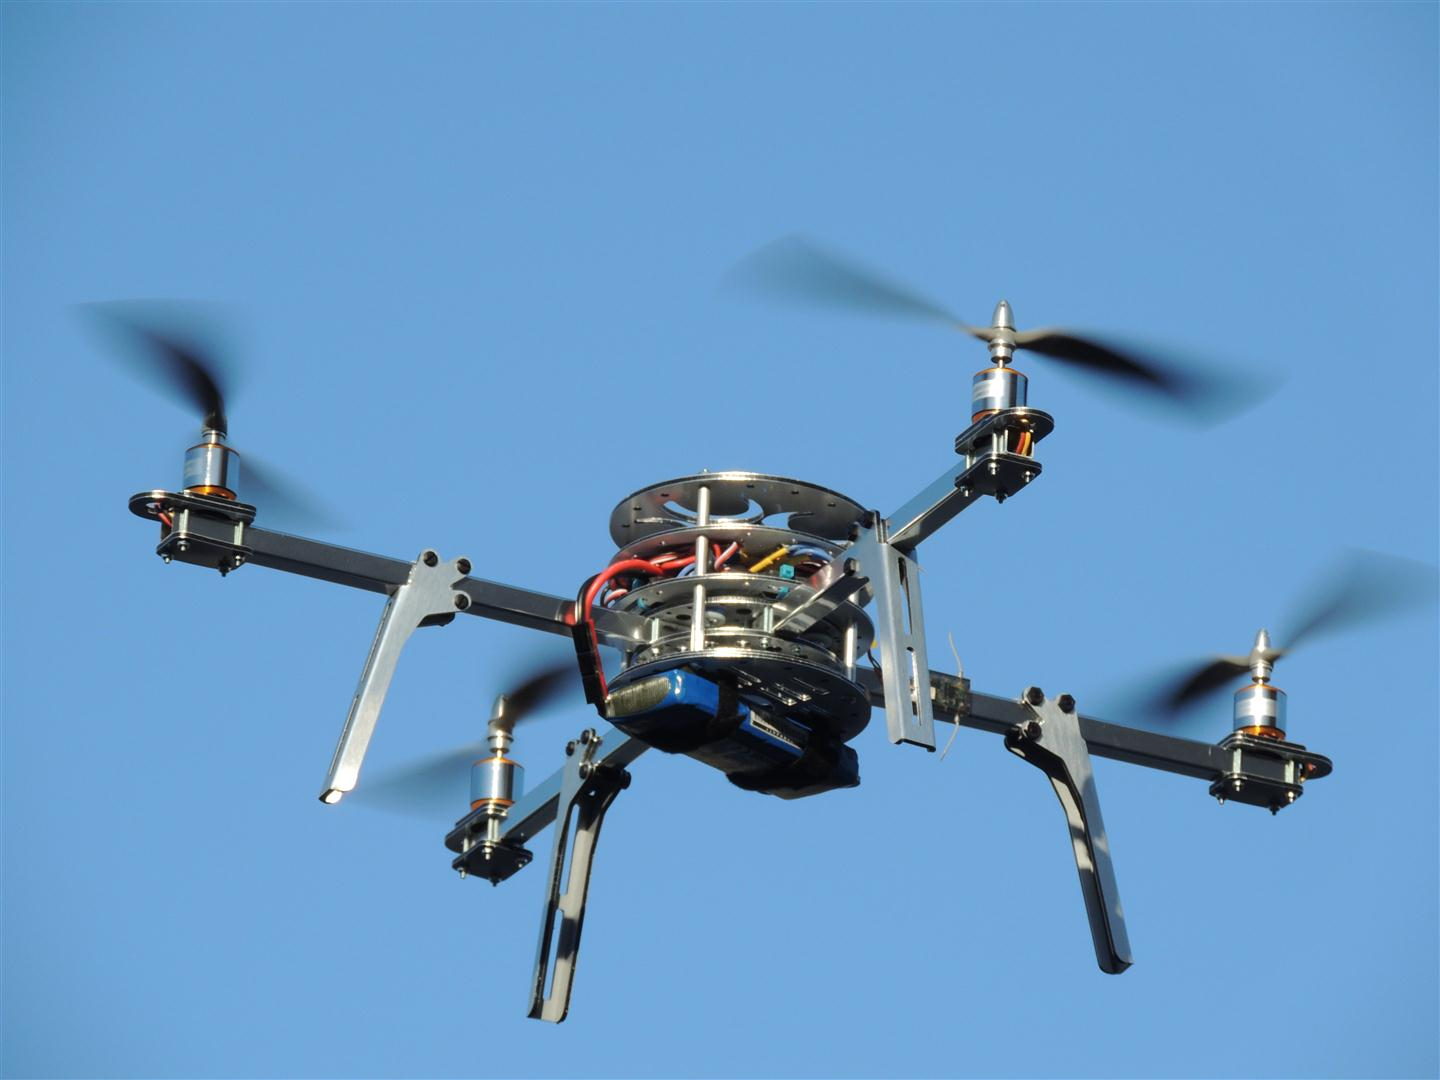
\includegraphics[width=0.7\textwidth]{pics/arduino-quadcopter.jpg}
    \caption*{\small \url{http://aeroquad.com/}}
  \end{figure}
\end{frame}

\begin{frame}{Raspberry Pi}
  \begin{center}
  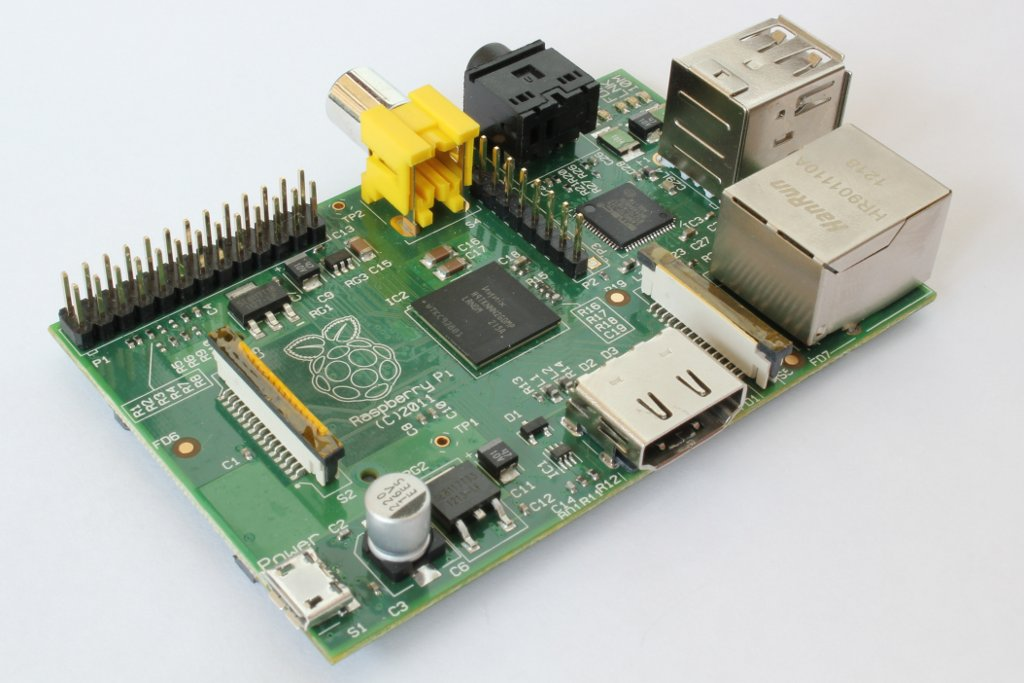
\includegraphics[width=.45\textwidth]{pics/raspberry-pi.jpg}
  \end{center}
  \vspace{-0.5cm}
  \begin{block}{}\centering
    Una placa de ordenador de bajo coste del tamaño de una tarjeta de
    crédito. Se puede instalar Debian (Raspbian) y tiene salida 1080p
    HDTV por HDMI.
  \end{block}
\end{frame}

\begin{frame}{Raspberry Pi: Servidor Torrent}
  \begin{figure}
    \centering
    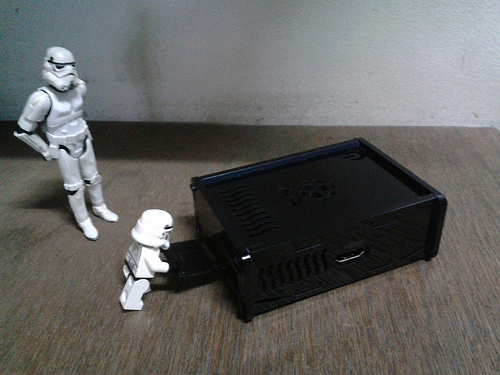
\includegraphics[width=0.5\textwidth]{pics/raspberry-pi-torrent-server.jpg}
    \caption*{\centering \small
      \url{http://eiosifidis.blogspot.com.es/2013/03/use-raspberry-pi-as-torrent-download.html}}
  \end{figure}
\end{frame}

\begin{frame}{Raspberry Pi: Luces de escritorio}
  \begin{figure}
    \centering
    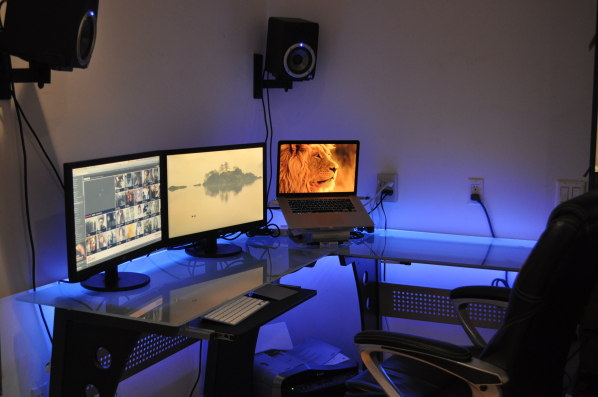
\includegraphics[width=0.6\textwidth]{pics/raspberry-pi-color-my-desk.jpg}
    \caption*{\centering \small
      \url{http://makezine.com/raspberry-pi-design-contest/rpidcg_005_color-my-desk/}}
  \end{figure}
\end{frame}

\begin{frame}{Raspberry Pi: Clúster de 64 nodos}
  \begin{figure}
    \centering
    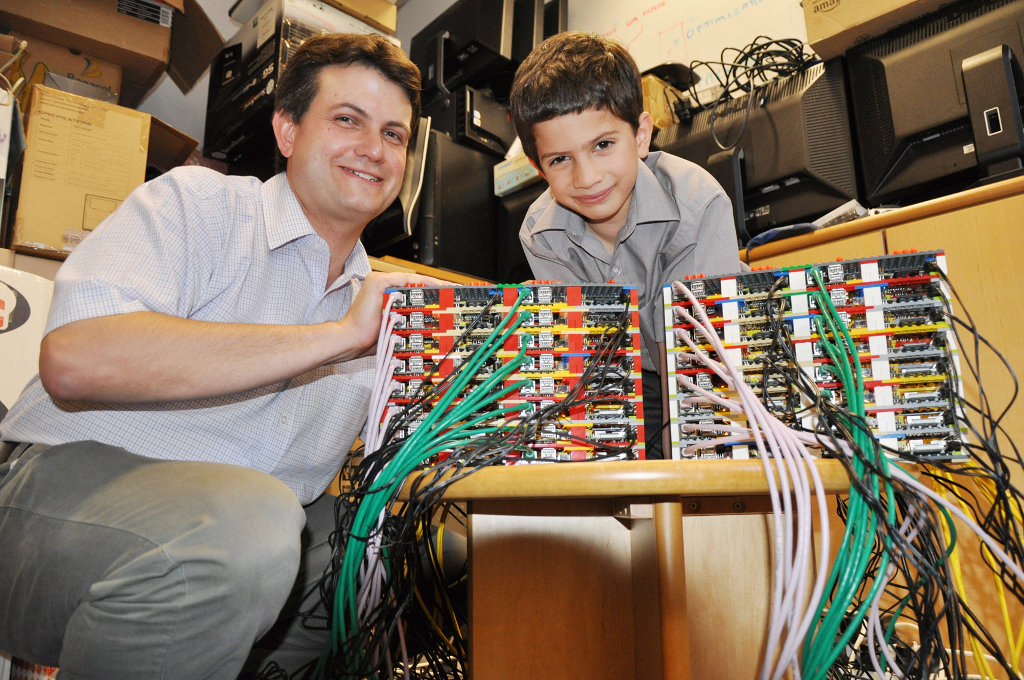
\includegraphics[width=0.7\textwidth]{pics/raspberry-pi-supercomputer.jpg}
    \caption*{\small \url{http://www.southampton.ac.uk/~sjc/raspberrypi/}}
  \end{figure}
\end{frame}

\section{Conclusión}

\ShowCurrentSection

\begin{frame}{Conclusión}
    \begin{block}{} \centering
      \normalsize El mundo es un lugar \structure{fantástico}, lleno
      de gente \structure{increíble} que trabaja en proyectos
      \structure{interesantes}. No seáis una gota más en un océano de
      mediocridad. Entregaos en cuerpo y alma a aquello que os
      apasione.
    \end{block}

    \begin{itemize} \itemsep0em
      \item Sólo si os gusta algo podréis llegar a ser
        \structure{realmente buenos}
      \item El futuro pertenece a los {\bf \structure{frikis}} (los de verdad)
  \item \structure{What if Money Did not Matter?}, de Alan Watts
      \item \structure{Everybody's Free To Wear Sunscreen}, de Baz Luhrmann
    \end{itemize}
\end{frame}


\end{document}

